\section{SonarCloud}
 \href{https://sonarcloud.io}{\textbf{SonarCloud}} è il prodotto leader per la \textbf{Continuous Code Quality} online ed è completamente gratuito per progetti open-source. Supporta tutti i principali linguaggi di programmazione, inclusi Java, C\#, JavaScript, C/C++ a molti altri. \textbf{SonarCloud} offre integrazioni end-to-end per i team che sfruttano le seguenti soluzioni nei loro processi di sviluppo:
\begin{itemize}
	\item GitHub
	\item Bitbucket Cloud
	\item Azure DevOps
\end{itemize}
Consente di effettuare le stesse analisi possibili in SonarQube \url{https://www.sonarqube.org/} senza però avere la necessità di installare il servizio in locale.
\subsection{SonarQube runner}
\textbf{SonarCloud} attualmente non triggera l'analisi automaticamente ma è necessario avviarla all'interno di uno script di Continuous Integration utilizzando uno tra i seguenti scanner disponibili:
\begin{itemize}
	\item Gradle - SonarScanner for Gradle
	\item MSBuild - SonarScanner for MSBuild
	\item Maven - use the SonarScanner for Maven
	\item Ant - SonarScanner for Ant
	\item anything else (CLI) - SonarScanner	
\end{itemize}
L'ultimo tra quelli elencati, \textbf{SonarScanner} può essere utilizzato quando nessuno degli altri risulta appropriato. La scelta è ricaduta su quest'ultimo visto che i progetti analizzati non utilizzano tutti lo stesso build automation tool. 
\subsection{Installazione SonarQube runner}
\textbf{SonarQube runner} è stato utilizzato su una macchina Ubuntu $16.04$ seguendo i passi riportati:
\begin{itemize}
	\item download dal maven repository utilizzando il seguente comando 
	\begin{verbatim}
		wget 
		http://repo1.maven.org/maven2/org/codehaus/sonar/runner/sonar-runner-dist/2.4/sonar-runner-dist-2.4.zip
	\end{verbatim}	
	\item unzip del file utilizzando il comando
	\begin{verbatim}
	unzip sonar-runner-dist-2.4.zip
	\end{verbatim}
	\item è necessario poi rendere eseguibile lo scanner presente nella directory bin utilizzando il comando 
	\begin{verbatim}
			sudo chmod u+x bin/sonar-scanner
	\end{verbatim}
	\item infine si crea un link simbolico in modo tale da poter eseguire lo scanner senza specificare ogni volta il path. Il comando da utilizzare è il seguente
	\begin{verbatim}
	 ln -s /opt/sonar-runner/bin/sonar-runner /usr/local/bin/sonar-runner
	\end{verbatim}
\end{itemize}
Risulta poi fondamentale modificare il file di configurazione \textit{sonar-scanner.properties} specificando il seguente campo:
\begin{verbatim}
	sonar.host.url=https://sonarcloud.io
\end{verbatim}

\subsection{Configurazione SonarCloud}
Affinché possa essere eseguita l'analisi è necessario configurare \textbf{SonarCloud}. Innanzitutto bisogna effettuare il log in ed è possibile farlo utilizzando l'account \textbf{gitHub} come mostrato in Figura \ref{fig:login}. Il secondo passo consiste nel creare una organizzazione, come mostrato in Figura \ref{fig:organizzazione}; si tratta di uno spazio all'interno del quale i membri di un team possono collaborare. Le organizzazioni possono essere create gratuitamente ma i progetti e le analisi risultano pubbliche. E\' possibile anche creare organizzazioni private anche se non gratuitamente. Una volta creata un'organizzazione è possibile, come mostrato in Figura \ref{fig:membri}, aggiungere membri al team specificando l'indirizzo e-mail o il nome utente utilizzato in gitHub dal collaboratore, e creare nuovi progetti. Si mostrano in Figura \ref{fig:nostraOrg} i membri dell'organizzazione realizzata per il progetto in esame.
\begin{figure}[htbp]
	\centering
	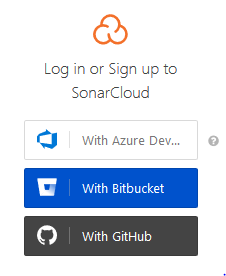
\includegraphics[scale=0.5, trim = 0cm 0cm 0cm 0cm, clip=true]{figSonarCloud/figLogInSonar.PNG}
	\caption{Schermata Log in SonarCloud}
	\label{fig:login}
\end{figure}

\begin{figure}[htbp]
	\centering
	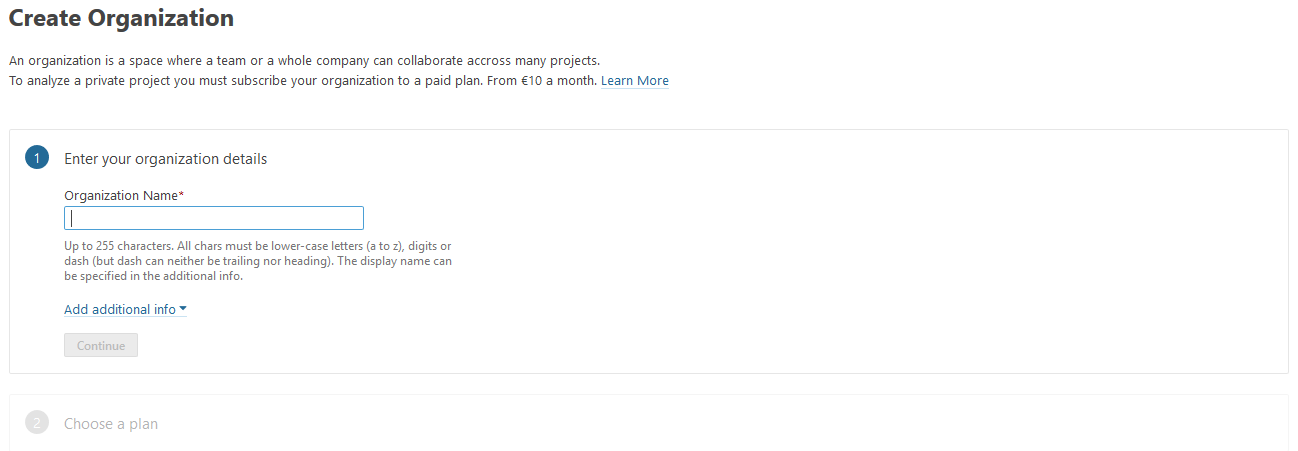
\includegraphics[scale=0.5, trim = 0cm 0cm 0cm 0cm, clip=true]{figSonarCloud/organizzazione.PNG}
	\caption{Creazione di una organizzazione in SonarCloud}
	\label{fig:organizzazione}
\end{figure}

\begin{figure}[htbp]
	\centering
	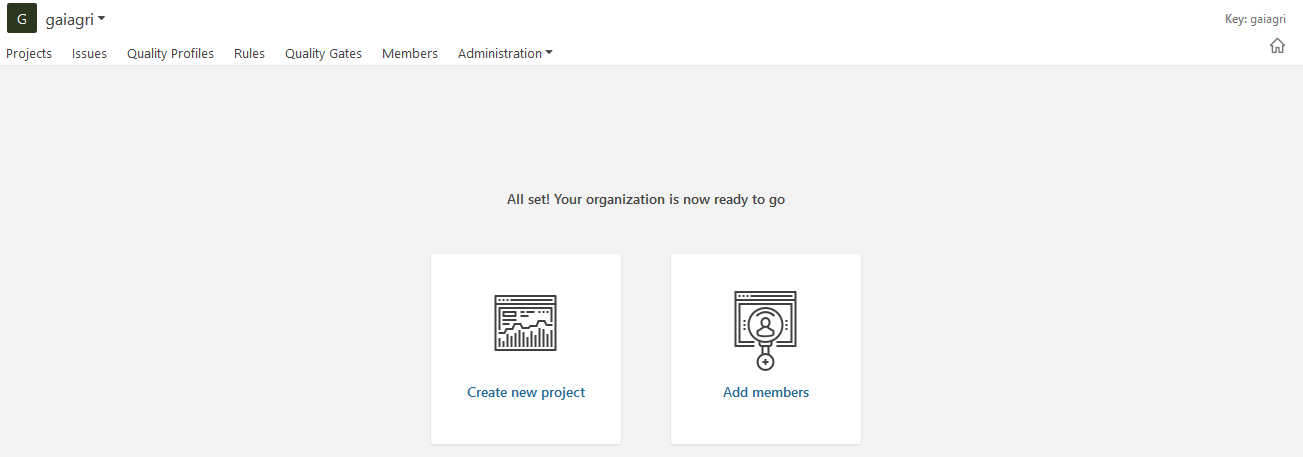
\includegraphics[scale=0.5, trim = 0cm 0cm 0cm 0cm, clip=true]{figSonarCloud/aggiuntaMembri.PNG}
	\caption{Aggiunta membri organizzazione e creazione progetto in SonarCloud}
	\label{fig:membri}
\end{figure}

\begin{figure}[htbp]
	\centering
	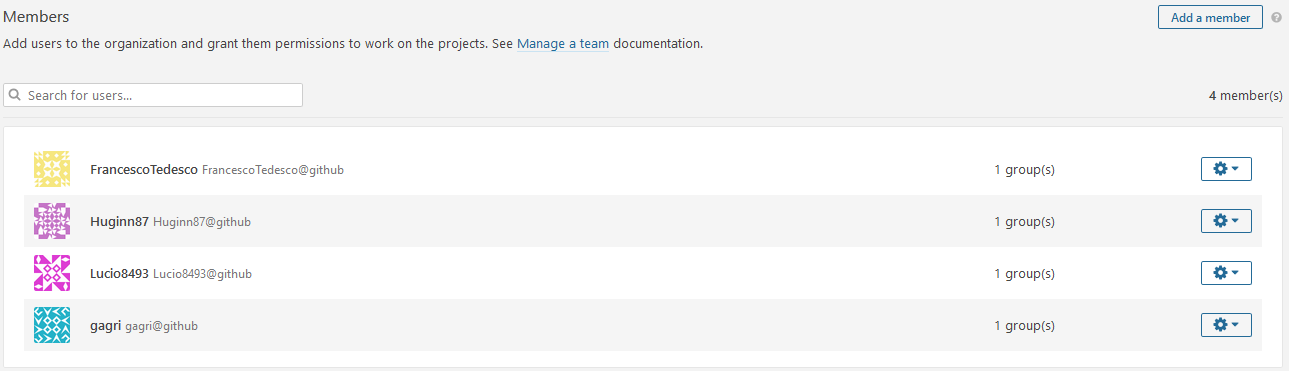
\includegraphics[scale=0.5, trim = 0cm 0cm 0cm 0cm, clip=true]{figSonarCloud/nostraOrganizzazione.PNG}
	\caption{Organizzazione progetto in esame}
	\label{fig:nostraOrg}
\end{figure}
A questo punto è possibile creare un nuovo progetto. E necessario specificare il nome dell'organizzazione, del progetto, che sarà lo stesso utilizzato in gitHub, ed una chiave che sarà univocamente assegnata a quel determinato progetto. Si mostra tale procedura in Figura \ref{fig:prog}.

\begin{figure}[htbp]
	\centering
	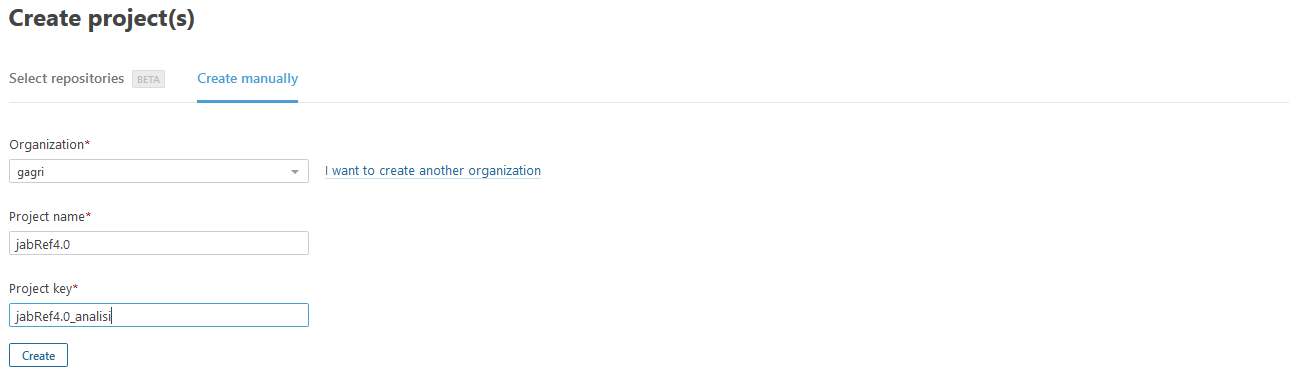
\includegraphics[scale=0.5, trim = 0cm 0cm 0cm 0cm, clip=true]{figSonarCloud/progetto.PNG}
	\caption{Creazione progetto sonarCloud}
	\label{fig:prog}
\end{figure}
Una volta creato il progetto, sarà mostrata una pagina che chiederà se si vuole generare un nuovo token oppure utilizzarne uno esistente. Il token è necessario al file di identificare l'utente che lancia l'analisi. L'associazione tra le informazioni (ossia organizzazione, chiave del progetto e token) e utente autorizzato a lanciare l'analisi, viene effettuata attraverso il file \textit{sonar-project.properties} che deve essere presente all'interno del progetto. In particolare le informazioni contenute risultano essere le seguenti:
\begin{itemize}
	\item 	sonar.projectKey: chiave del progetto
	\item 		sonar.organization: nome dell'organizzazione
	\item 	sonar.host.url: nel caso in cui si utilizza sonarCloud è necessario specificare l'URL di quest'ultimo ossia \url{https://sonarcloud.io}. Nel caso di utilizzo di SonarQube in locale, bisognerebbe specificare \url{http://localhost:9000}
	\item 	sonar.login: token fornito in fase di creazione del progetto
	\item sonar.sources: directory contenete i sorgenti
	\item sonar.java.binaries: directory contenete i binari
	\item sonar.language: linguaggio di programmazione del progetto in analisi
\end{itemize}

A questo punto, basta lanciare il comando 
\begin{verbatim}
sonar-runner
\end{verbatim}
per avviare l'analisi ed una volta che questa è terminata il risultato sarà visualizzabile online come mostrato a titolo esemplificativo in Figura \ref{fig:analisi}.
	
\begin{figure}[htbp]
	\centering
	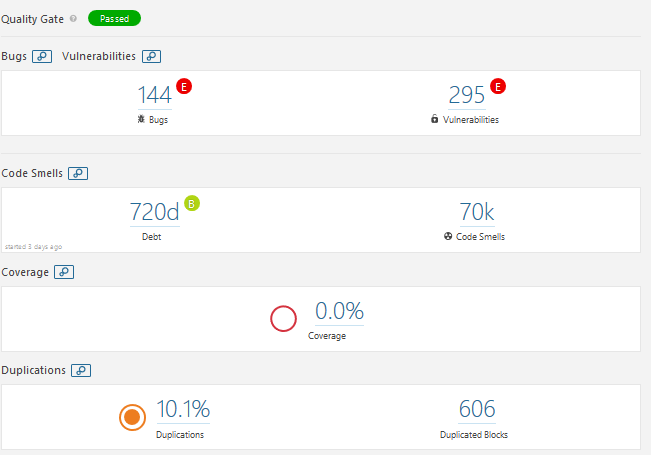
\includegraphics[scale=0.5, trim = 0cm 0cm 0cm 0cm, clip=true]{figSonarCloud/analisi.PNG}
	\caption{Esempio risultato analisi SonarCloud}
	\label{fig:analisi}
\end{figure}